\begin{figure}[h!]
    \centering
    
\includegraphics[width=0.8\linewidth]{pics/express_logo.png}
    \caption{Express.js Logo}
    \label{fig:enter-label}
\end{figure}
Express.js ist ein Node.js-Framework, das erstmals im November 2010 veröffentlicht wurde. Trotz seiner minimalistischen Ausrichtung zeichnet sich Express, durch seine Erweiterbarkeit und Vielseitigkeit aus. Dies wird durch eine Fülle von Libraries und Modules ermöglicht, die in das Framework integriert sind oder von der Entwicklergemeinschaft entwickelt wurden. Diese Ressourcen erleichtern die Bewältigung komplexer Aufgaben, wie die Handhabung von Cookies, Sitzungsverwaltung, Benutzeranmeldung und viele weitere Funktionen, die für moderne Webanwendungen von entscheidender Bedeutung sind.
\newline
Eine der architektonischen Merkmale von Express ist sein Middleware-Konzept. Dieses ermöglicht die Verarbeitung von HTTP-Anfragen in Schichten. Jede Middleware-Funktion kann spezifische Aufgaben übernehmen und ist in der Lage, Requests und Responses zu modifizieren oder zu ergänzen, bevor sie an die nächste Middleware-Funktion weitergeleitet werden. Dies bietet eine hohe Flexibilität und Kontrolle über den Anfragen- und Antwortfluss in einer Express-Anwendung.
\cite{Express_js_Introduction}

\subsubsection{Routing}
Das Routing, im Kontext von Webanwendungen, spielt eine entscheidende Rolle bei der Bestimmung, wie die Anwendung auf eine Clientanfrage in Bezug auf einen spezifischen Endpoint reagiert. Dieser Prozess ist von essenzieller Bedeutung, um Anfragen an die korrekte Ressource oder den gewünschten Endpunkt innerhalb der Anwendung zu leiten. Um diesen Zweck zu erfüllen, sind zwei entscheidende Informationen erforderlich: der Pfad und die HTTP-Methode.
\newline
Der Pfad definiert die URL-Struktur, anhand derer die Anfrage geroutet wird. Dies ermöglicht die Identifikation des gewünschten Endpunkts oder der Ressource innerhalb der Anwendung. Die HTTP-Methode gibt an, welche Aktion auf dem spezifizierten Pfad ausgeführt werden soll. Es ist wichtig anzumerken, dass eine Route innerhalb einer Webanwendung mehrere HTTP-Funktionen besitzen kann. Dies bedeutet, dass eine bestimmte URL-Ressource oder ein Endpoint für verschiedene HTTP-Anfragen unterschiedliche Reaktionen bieten kann. Dies ermöglicht die Implementierung von CRUD-Operationen (Create, Read, Update, Delete) für bestimmte Ressourcen und bietet somit eine flexible und mächtige Möglichkeit zur Interaktion mit der Anwendung.
\cite{Express_js_basic_routing}
\cite{Express_js_routing}

\subsubsection{Middleware}
Middleware Funktionen haben Zugriff auf das Request-Object (\textbf{req}), das Response-Object (\textbf{res}) und auf die \textbf{next} Funktion. Mittels next kann nach Abschluss einer Middleware die nächste Middleware aufgerufen werden, dafür gibt es zwei Möglichkeiten.
\begin{itemize}
    \item ohne Übergabeparameter
        \newline
        Durch das einfache Aufrufen von next ohne Übergabeparameter wird der Request unverändert weitergeleitet und die Ausführung des Codes wird in der nächsten geeigneten Middleware oder Route fortgesetzt. Dieses Vorgehen ermöglicht die nahtlose Verarbeitung von Anfragen und die Kontinuität der Anwendungslogik, ohne den Request zu modifizieren oder zu unterbrechen.
    \item mit Übergabeparameter
        \newline
        In Bezug auf die Übergabeparameter existieren zwei verschiedene Optionen. Die Erste besteht darin, dass, wenn die Zeichenfolge 'route' als Parameter übergeben wird, sämtliche Middleware-Funktionen ignoriert werden, und stattdessen nach einer passenden Route gesucht wird. Die Zweite Möglichkeit besteht darin, dass ein anderer Wert als 'route' übergeben wird. Dabei behandelt Express diesen Aufruf als Fehler und überspringt jegliche Middleware- und Route-Funktionen, die keine Fehler zurückgeben. Dieser Ansatz gewährleistet die angemessene Verarbeitung von Anfragen und ermöglicht die gezielte Steuerung des Anwendungsflusses, wobei die Behandlung von Fehlern oder das Überspringen bestimmter Schritte je nach Bedarf erfolgt.
\end{itemize}
In einer Express Applikation ist es möglich 5 verschiedene Arten von Middleware einzubinden.

\begin{itemize}
    \item \textbf{Application-Level Middleware}
        \newline
        Diese Middleware wird als Instanz des App-Objekts eingebunden, indem man entweder app.use() oder app.METHOD() benutzt. Bei einer Method Funktion, kann man die drei HTTP-Methoden get, put oder post benutzen. Diese müssen allerdings in Kleinbuchstaben geschrieben werden.
        \newline
        Im folgenden Codebeispiel wird eine Middleware-Funktion implementiert, die bei jedem Request an die App das aktuelle Datum ausgibt. Nachdem das Datum auf der Konsole ausgegeben wird, wird next() aufgerufen, wodurch der Request unverändert bleibt. Falls der Pfad der Syntax "user/:id" entspricht, wird die Ausführung an die erste Middleware weitergeleitet. Wenn die ID den Wert Null aufweist, wird next mit dem Übergabeparameter "route" aufgerufen, der auf die nächste Route verweist. In diesem Fall würde die Middleware "special" als Antwort zurückliefern. Wenn die ID jedoch von null verschieden ist, wird next ohne Übergabeparameter aufgerufen, und der Request wird an die nächste Middleware-Funktion weitergeleitet. In diesem Fall würde die Antwort "regular" lauten.
        \newline
        \begin{lstlisting}
            const express = require('express')
            const app = express()

            app.use((req, res, next) => {
                console.log('Time:', Date.now())
                next()
            })
    
            app.get('/user/:id', (req, res, next) => {
                if (req.params.id === '0') next('route')
                else next()
            }, (req, res, next) => {
                res.send('regular')
            })

            app.get('/user/:id', (req, res, next) => {
                res.send('special')
            })
        \end{lstlisting}
    \item \textbf{Router-Level Middleware}
        \newline
        Diese Middleware arbeitet genau gleich wie die Application-Level Middleware, mit dem Unterschied, dass diese eine Instanz des express.Router() ist. Der Nutzen dieser Art von Middleware ist, eine Modularität zu erzeugen, welche es möglich macht, eine Anwendung in kleinere Teile aufzuteilen. Dadurch hat man die Möglichkeit, ein eigenes Untersystem, wie im unten gezeigten Codebeispiel für alle User-Requests zu erstellen. Im folgenden Beispiel werden alle /user Anfragen an den userRouter weitergeleitet und in einem externen File beantwortet.
        \newpage
        \begin{lstlisting}
            const userRouter = require('./userRouter')
            
            app.use('/user', userRouter)
        \end{lstlisting}

        \begin{lstlisting}
            router.get('/getAll', (req, res) => {
                res.send('Alle User')
            }
        \end{lstlisting}
    \item \textbf{Error-Handling Middleware}
        \newline
        Die Error-Handling Middleware funktioniert auf die gleiche Weise wie die oben genannten Middlewares, mit dem kleinen Unterschied, dass 4 Argumente übergeben werden können.
        \begin{lstlisting}
            app.use((err, req, res, next) => {
                console.log(err.stack)
                res.status(500).send('Etwas ist schief gelaufen')
            }
        \end{lstlisting}
    \item \textbf{Built-In Middleware}
        \newline
        Ab Version 4.x verwendet Express nicht mehr Connect und frühere Middleware Funktionen sind in separaten Modulen (third-party middlewares) ausgelagert. Folgende Built-In Middleware-Funktionen sind noch in Express verfügbar:
        \begin{itemize}
            \item \textbf{express.static}
                \newline
                Zur Anzeige von statischem Content, wie zum Beispiel HTML oder Bildern
            \item \textbf{express.json}
                \newline
                Zur Übersetzung von ankommenden JSON requests.
            \item \textbf{express.urlencoded}
                \newline
                Zur Übersetzung von ankommenden URL requests.
        \end{itemize}
    \item \textbf{Third-Party Middleware}
        \newline
        Diese Middleware hat die Aufgabe, einer Express Applikation mehr Funktionalität zu verleihen. Dabei lädt man mittels NPM die gewünschte Middleware aus dem Internet herunter und kann diese anschließend in sein Backend einbauen.
        \begin{lstlisting}
            const express = require('express')
            const app = express()
            const cookieParser = require('cookie-parser')

            app.use(cookieParser())
        \end{lstlisting}
        \newpage
        Es gibt folgende Third-Party Middlewares:\newline
        \begin{figure}[h!]
            \centering
            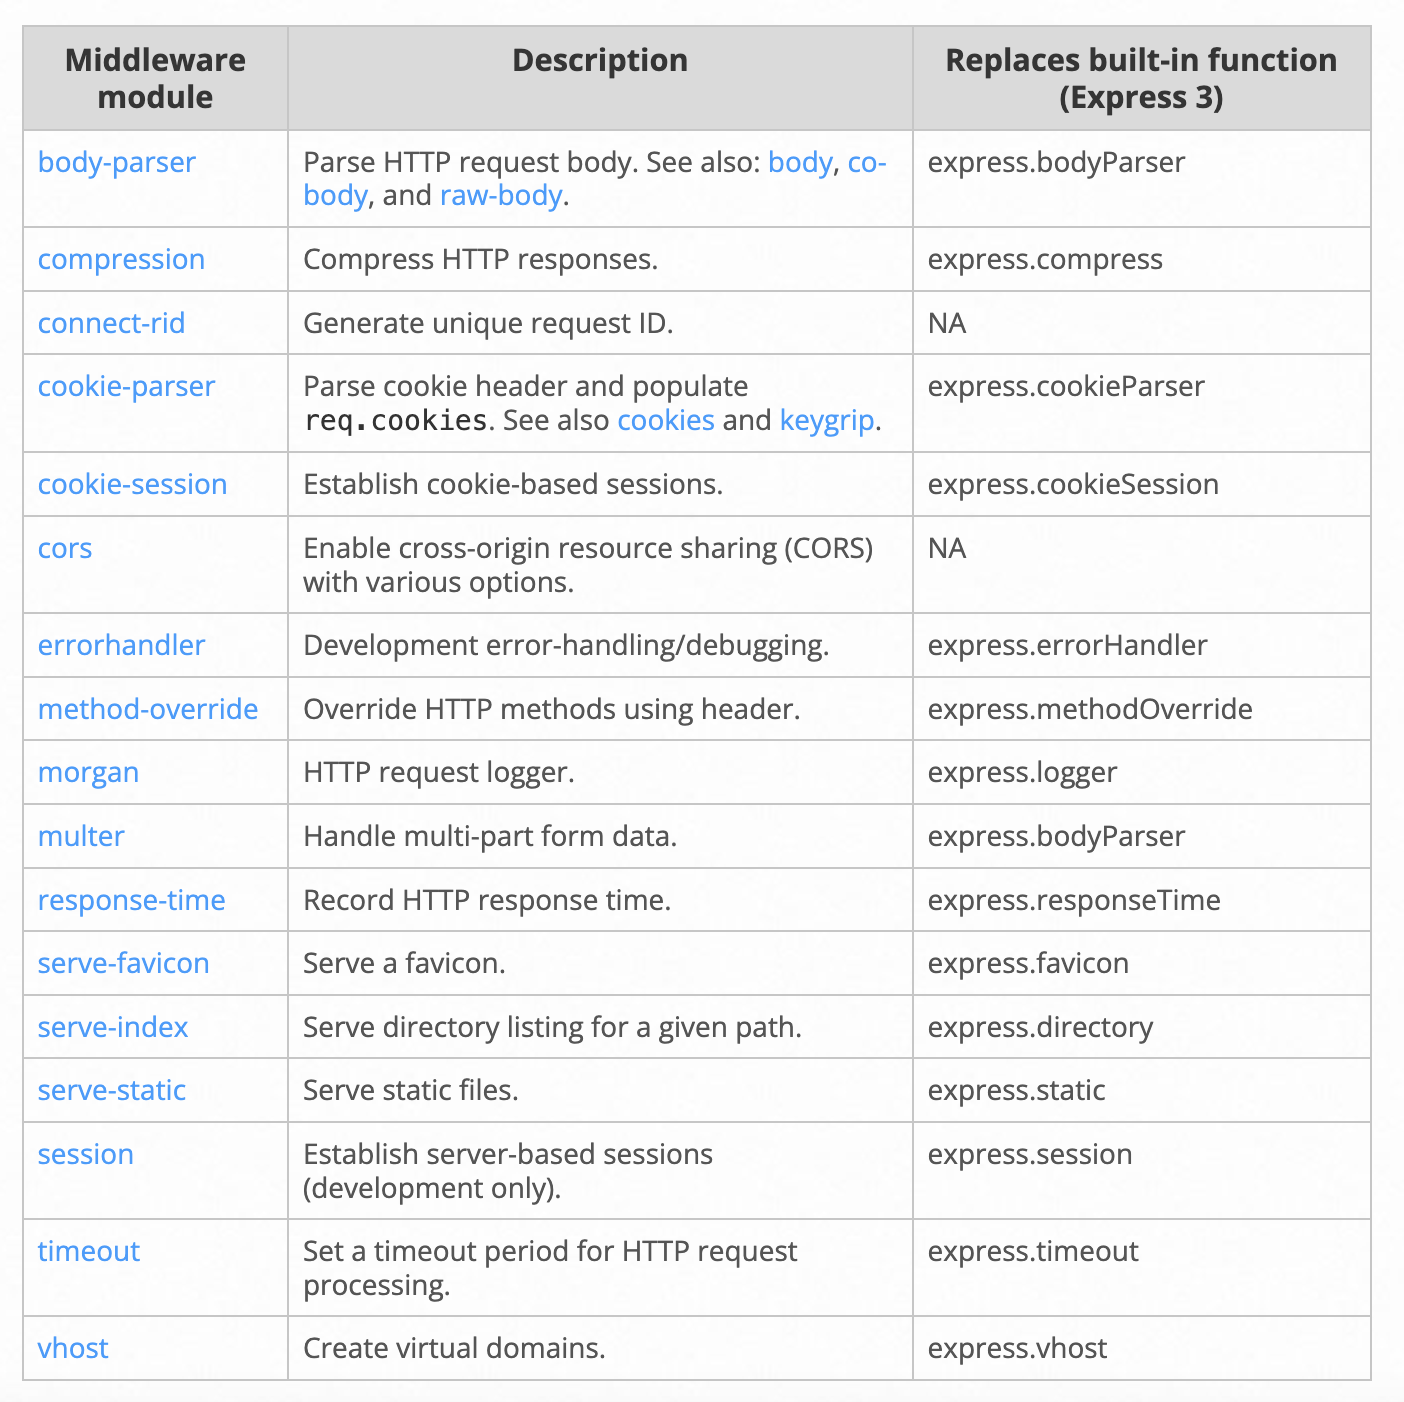
\includegraphics[width=0.45\textwidth]{pics/Third-Party-Middleware.png}
            \caption{Third Party Middlewares}
            \cite{Express_js_third_party_middlewares}
            \label{fig:enter-label}
        \end{figure}
\end{itemize}
\cite{Express_js_writing_middleware}
\cite{Express_js_using_middleware}
\cite{Express_js_middleware_help_1}

\subsubsection{Überschreiben der Express API}
Die Express API besteht aus dem Request und Response Objekt. Diese besitzen verschiedene Funktionen und Übergabeparamter. Man kann die Funktionen der beiden Objekte auf zwei verschiedenen Ebenen verändern. Zum einen kann man diese global, mittels \textbf{express.request} und \textbf{express.response} verändern und zum anderen Applikationsspezifisch, durch den Aufruf von \textbf{app.request} und \textbf{app.response}. Eine globale Änderung, wirkt sich auf alle Express-Applikationen im selben Prozess aus, Applikationsspezifische Änderungen können erst nach Erstellung einer neuen App durchgeführt werden und gelten dementsprechend nur für das spezifische Objekt. 

\textbf{Überschreiben von Methoden}
\newline
Um die Express API überschreiben zu können, wird an eine bestehende Funktion eine neue, eigens erstellte Methode angehängt.
\begin{lstlisting}
    app.response.sendStatus = function(statusCode, type, message) {
        return this.contentType(type)
            .status(statusCode)
            .send(message)
    }
\end{lstlisting}
In dem oben gezeigten Fall wurde die sendStatus Funktion überschrieben und es wird von nun an eine eigens erstellte Response zurückgegeben. Die überschriebene Funktion kann nun auf folgende Weise aufgerufen werden.
\begin{lstlisting}
    res.sendStatus(404, 'application/json', '{"error":"resource not found"}            
\end{lstlisting}

\textbf{Überschreiben von Properties}
\newline
Properties in der Express API werden in folgende 2 Kategorien eingeteilt: 
\begin{itemize}
    \item Assigned Properties
    \item Defined as Getters
\end{itemize}
Properties aus Kategorie 1, sind dynamisch zugewiesene Eigenschaften und können daher nicht überschrieben werden. Properties aus der 2. Kategorie können mittels Express API extensions API überschrieben werden. Der folgende Code zeigt, wie man den Wert des \textbf{req.ip} Properties verändern kann. In diesem Fall wird nur die Client-IP aus dem Request-Header ausgegeben.
\begin{lstlisting}
    Object.defineProperty(app.request, 'ip', {
        configurable: true,
        enumerable: true,
        get() { return this.get('Client-IP') }
    }
\end{lstlisting}

\textbf{Überschreiben von Prototypes}
\newline
Um die Express API bereitzustellen, müssen die Request und Response Objekte von derselben Prototypenkette abstammen. Standardmäßig sind \textbf{http.IncomingRequest.prototype} und \textbf{http.ServerResponse.prototype} für die Anfragen und Antworten zuständig. Das Überschreiben der Prototypen sollte, außer wenn es nicht anders möglich ist, nur auf der App-Ebene durchgeführt werden.
\begin{lstlisting}
    Object.setPrototypeOf(Object.getPrototypeOf(app.request), FakeRequest.prototype)
    Object.setPrototypeOf(Object.getPrototypeOf(app.response), FakeResponse.prototype)
\end{lstlisting}
In dem oben gezeigten Beispiel wird der Prototyp von den http.IncomingRequest/ http.ServerResponse auf FakeRequest/FakeResponse umgestellt.
\cite{Express_js_overriding_api}

\subsubsection{Fehlerbehandlung}
Express.js ist mit einer per default definierten Fehlerbehandlung ausgestattet, es ist dementsprechend nicht notwendig eine eigene zu implementieren. In einem Backend ist es essenziell, alle Fehler in der Laufzeit abzufangen, um ein Abstürzen des Servers zu vermeiden. Bei einem nicht asynchronen Code innerhalb einer Middleware oder einer Route, muss man keinen zusätzlichen Arbeitsaufwand aufwenden, da Express den Fehler von selbst auffängt und anschließend verarbeitet. Bei einem asynchronen Code ist dies anders. In diesem Fall muss next() aufgerufen werden und der Fehler wird in einer anderen Funktion aufgefangen und verarbeitet. Ab der Express Version 5, rufen Middlewares und Routes bei einem asynchronen Code automatisch next() auf, falls ein Fehler auftritt.
\begin{lstlisting}
    app.get('/user/:id', async (req, res, next) => {
        const user = await getUserById(req.params.id)
        res.send(user)
    }
\end{lstlisting}
Im oben gezeigten Beispiel ist die Fehlerbehandlung von Express automatisch implementiert. Falls die Funktion getUserById einen Fehler auswirft, wird automatisch next aufgerufen. Der Übergabeparameter beinhaltet entweder den übergebenen Fehler oder den abgelehnten Wert. Falls keines dieser beiden von der Funktion übergeben wird, wird ein default Fehlerobjekt übergeben.

\textbf{Default Fehlerbehandlung}
\newline
Express stellt eine bereits eingebaute Fehlerbehandlung zur Verfügung, welcher sich um jeglichen Fehler in der Applikation kümmert. Diese Fehlerbehandlung muss lediglich am Ende des Middleware-Funktionen-Stacks eingebunden werden. Falls man nun mittels next einen Fehler übergibt, behandelt diese Middleware den Fehler und gibt diesen am Client aus. Tritt ein Fehler auf, werden folgende Informationen im Response Objekt gespeichert:
\begin{itemize}
    \item res.statusCode
        \newline
        Falls dieser Wert außerhalb des 400 und 500 Statuscodebereiches ist, wird automatisch der Fehlercode auf 500 (Server Internal Error) gesetzt.
    \item res.statusMessage
        \newline
        Wird anhand des Fehlercodes gesetzt.
    \item Body
        \newline
        Dies ist der HTML Code der Fehlermessage in einer Produktionsumgebung. Falls dies nicht der Fall ist, heißt das Objekt \textbf{err.stack}.
    \item Header
        \newline
        Alle Header die im \textbf{err.headers} Objekt vorhanden sind.
\end{itemize}
In dem Fall, dass man mittels next einen Fehler aufrufen möchte, man jedoch bereits eine Response an den Client zu schicken begonnen hat, beendet Express die Verbindung und lässt den Request fehlschlagen.

\textbf{Fehlerbehandlung selbst schreiben}
\newline
Wie bereits dargestellt, besteht die Middleware aus 4 Parametern (err, req, res, next). Zu beachten ist, dass die Fehlerbehandlung die letzte implementierte Middleware sein muss. Man kann die Response auf verschiedenste Arten gestalten, zum Beispiel eine HTML-Seite, einen einfachen Fehlertext oder einen JSON-String zurück liefern.
\cite{express_js_error_handling}

\textbf{Debugging}
\newline
Debugging heißt wörtlich übersetzt "Entfernen von Fehlern". Allerdings ist mit Debugging ein mehrstufiger Prozess gemeint, mit dem man einen Fehler identifizieren, die Ursache des Problems herausfinden und anschließend den Fehler beheben beziehungsweise übergehen kann.
\cite{debugging_allgemein}
\newline
Um in Express debuggen zu können und alle internen Ausgaben zu sehen, muss man lediglich die \textbf{DEBUG} Umgebungsvariable auf \textbf{express:*} setzen, wenn man die App startet.
\begin{verbatim}
// Für MacOS
DEBUG=express:* node index.js

// Für Windows
set DEBUG=express:* & node index.js
\end{verbatim}
Man hat nun die Möglichkeit, weitere Optionen für das Debuggen zu definieren.
\begin{center}
    \begin{tabular}{||c c||} 
        \hline
        Befehl & Beschreibung \\ [0.5ex] 
        \hline\hline
        DEBUG & Enables/disables specific debugging namespaces \\ 
        \hline
        DEBUG\_COLORS & Whether or not to use colors in the debug output \\
        \hline
        DEBUG\_DEPTH & Object inspection depth \\
        \hline
        DEBUG\_FD & File descriptor to write debug output to \\
        \hline
        DEBUG\_SHOW\_HIDDEN & Shows hidden properties on inspected object \\ [1ex] 
        \hline
    \end{tabular}
\end{center}
\cite{Express_js_third_party_middlewares}

Die Identifizierung von Fehlern und die Debugging-Funktionalität in Visual Studio Code (VS-Code) bieten die Möglichkeit, nicht nur die internen Ausgaben zu erhalten, sondern auch eigens verfasste Funktionen zu überprüfen. Diese Funktionalität wird durch das Setzen von Breakpoints ermöglicht, die einfach neben der Zeilennummer platziert werden. Der Debugger wird daraufhin in der Menüleiste gestartet. Das Starten des Debuggers bewirkt, dass VS-Code die Anwendung ausführt und den Debugger aktiviert. Bei Aufruf der zu überprüfende Funktion pausiert das Programm an der Stelle, an der zuvor der Breakpoint gesetzt wurde. Hierbei stehen sämtliche existierenden Variablen zur Inspektion zur Verfügung und der Code kann schrittweise durchlaufen werden.
\newline
Eine zusätzliche und oft einfachere Methode, um den eigenen Code zu debuggen, besteht darin, mithilfe von \textbf{console.log} Variablen auszugeben. Auf diese Weise kann überprüft werden, warum der Code fehlerhaft ist und welche Werte in den Variablen enthalten sind.
\cite{express_js_debugging}